\section{Methods \& Materials} \label{methods}
\subsection{Tagging \& pinning}
Ants were selected from their nests based on their relatively large size and high activity. Before being placed in the set-up described below, each individual ant was marked with a distinct pattern of coloured paint spots (Humbrol Enamel, Hornby Hobbies Ltd, Kent, UK) on its thorax and abdomen for posterior identification. Tagged ants were left in a box with inside walls covered in fluon (ASC 109, Blades Biological Ltd, Edenbridge, UK) for at least 30 minutes before pinning for the paint to dry. Ants were then anaesthetized with ice and placed under a microscope (210444, Olympus Corporation, Tokyo, Japan). A fine minutien pin (0.1 mm diameter, 1 cm length; Fine Science Tools GmbH, Heidelberg, Germany), with the top third bent around 45$\degree$ was attached to the most posterior segment of their thorax using fast dry UV glue (5SF-MC12/6, 5 Second Fix). Painted and pinned ants were left inside the same fluoned box until being restrained in the virtual reality set-up.

\subsection{Virtual reality setup}
In short, our virtual reality (VR) system consisted on a walking platform which movement was recorded and in turn changed the coordinates of the projected virtual world accordingly. This created a closed-loop between the ants’ movement and the visual stimuli, allowing them to navigate in a virtual environment (figure \ref{fig:setup}).

To reduce the presence of visual cues between the ant and the projection, a 3D printed custom made floor was placed above the polystyrene ball, with a 2 cm diameter hole in the centre where the ant was placed (figure \ref{fig:setup}). 

\begin{figure}
\centering
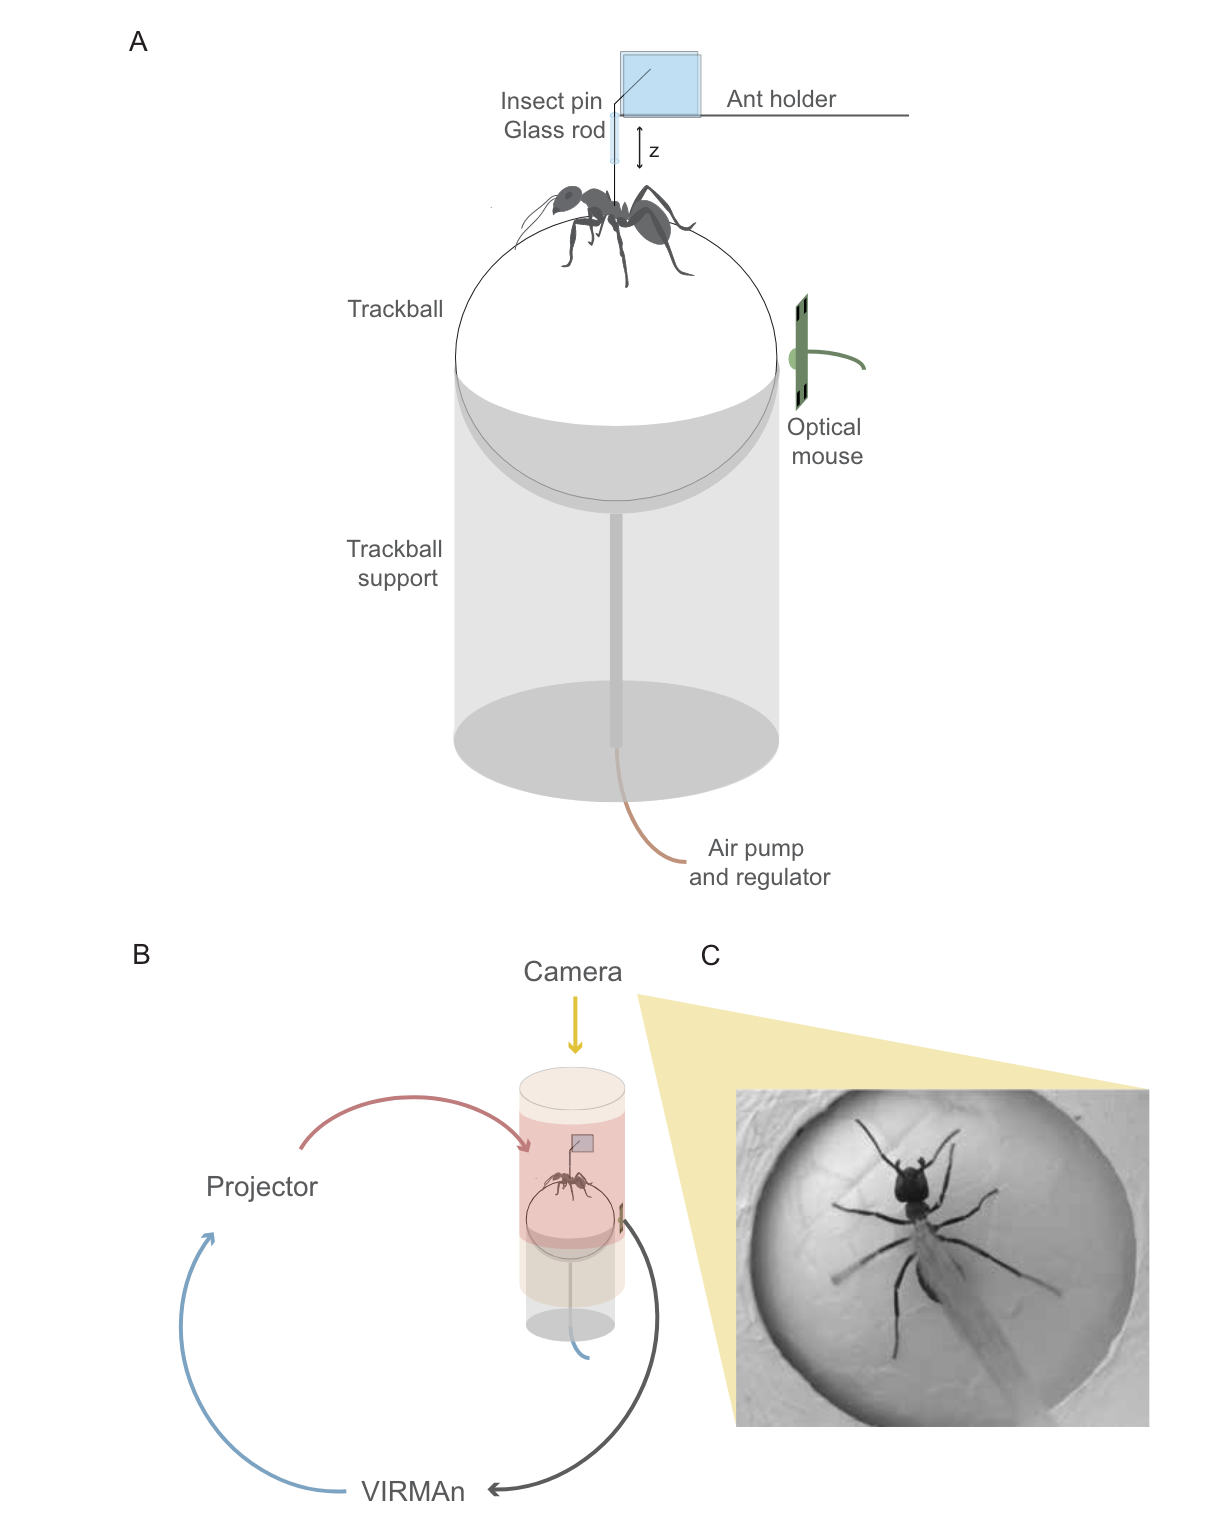
\includegraphics[width=\hsize]{figures/setup.png}
\caption{\textbf{Schematic diagram of the virtual reality paradigm}. A) Wood ants are placed on top of a polystyrene ball (trackball), seating on a metallic cup (trackball support) perforated inside to allow pressure regulated air flow from an air pump to support the trackball. The ant is restrained by an insect pin glued to the posterior portion of the thorax. The insect pin is kept in place by a glass rod and two custom made plastic structures that allow the ant to move up and down (z) but not rotate on top of the ball. As the ant walks, the air supported trackball moves underneath, which is recorded by an optical mouse. B) The optical mouse is connected to a computer running the Matlab package VIRMEn. VIRMEn creates a virtual world and changes it according to the optical mouse recordings. The virtual world is displayed to the ant through a projector connected to the same computer onto a tracing paper cylinder surrounding the ant, trackball and support. C) A camera placed above the set-up records the ant at all times. A portion of the trackball is covered by a custom made white floor to reduce the presence of visual cues between the ant and the virtual world.
}
\label{fig:setup}
\end{figure}



